\documentclass[12pt]{article}
\usepackage[a4paper, total={6.5in, 9.4in}]{geometry}
\usepackage{graphicx}
\graphicspath{ {./images/output/} }
\usepackage{caption}
\usepackage[english]{babel}
\usepackage{titling}
\usepackage{float}
\usepackage{amsmath}
\usepackage{minted}
\usepackage{multicol}
\usepackage{array}
\usepackage{setspace}
\usepackage{placeins}
\usepackage{parskip}

% \usepackage{lipsum}

\title{Experiment 2\\
\textbf{Experiment on Control Controllability and Observability of a System}}
\author{}
\date{}

\pagenumbering{gobble}
\begin{document}
\vspace*{\fill}
\begin{center}

    \emph{Heaven's Light is Our Guide} \\
    \textbf{Rajshahi University of Engineering and Technology} \\

    \begin{figure}[H]
        \centering
        
\includegraphics[scale=.34]{images/RUET_logo.png}
        \label{fig:ruet_logo}
    \end{figure}
    \vspace{5mm}

    \textbf{Course Code}\\
    MTE 4118\\
    \vspace{3mm}
    \textbf{Course Title}\\
    Control System and Robotics Sessional

    \vspace{5mm}
    \textbf{Experiment Date:} {July 22, 2025},\\
    \textbf{Submission Date:} {August 19, 2025}\\

    \vspace{5mm}
    \textbf{Lab Report 2: \\
        Experiment on Control Controllability and Observability of a System}

    \vspace{15mm}

    \begin{tabular}{c|c}
        \textbf{Submitted to}      & \textbf{Submitted by} \\
        Md. Sakib Hassan Chowdhury & Md. Tajim An Noor     \\
        Lecturer                   & Roll: 2010025         \\
        Dept of MTE, RUET          &                       \\
    \end{tabular}

\end{center}
\vspace*{\fill}


\pagebreak

\tableofcontents

\pagebreak
\pagenumbering{arabic}
\maketitle

\vspace{-5em}

\section*{Objectives}
\addcontentsline{toc}{section}{Objectives}
\begin{enumerate}
  \item Explain controllability and observability in state-space systems.
  \item Use MATLAB to test these properties for a given system.
  \item Analyze results using controllability and observability matrices.
\end{enumerate}

\section*{Theory}
\addcontentsline{toc}{section}{Theory}
In control systems, the state-space approach models a system using a set of state variables that capture the internal condition of the system at any moment~\cite{Ogata, Nise}. These state variables, together with the system's inputs and outputs, are related through mathematical equations that describe the system's dynamic behavior:

\begin{align*}
  \dot{x}(t) & = A x(t) + B u(t) \\
  y(t)       & = C x(t) + D u(t)
\end{align*}

where:
\begin{itemize}
  \item $x(t)$ is the vector of state variables,
  \item $u(t)$ is the input vector,
  \item $y(t)$ is the output vector,
  \item $A$, $B$, $C$, and $D$ are matrices that define the relationships between states, inputs, and outputs.
\end{itemize}

\textbf{Controllability:} \\
A system is controllable if it is possible to drive the system from any initial state to any final state within a finite time using suitable inputs~\cite{Ogata}. To determine controllability, we construct the controllability matrix:

\[
  \mathcal{C} = \begin{bmatrix} B & AB & A^2B & \cdots & A^{n-1}B \end{bmatrix}
\]

If this matrix has full rank (equal to the number of state variables), the system is considered controllable.\\

\textbf{Observability:} \\
A system is said to be observable if the internal state variables can be determined from the system's outputs and known inputs over time~\cite{Nise}. To assess observability, we construct the observability matrix:

\[
  \mathcal{O} = \begin{bmatrix} C \\ CA \\ CA^2 \\ \vdots \\ CA^{n-1} \end{bmatrix}
\]

If this matrix has full rank (equal to the number of state variables), the system is considered observable.

\subsection*{Experiment Matrix Calculation}
\addcontentsline{toc}{subsection}{Experiment Matrix Calculation}
The experiment matrix is constructed to analyze the controllability and observability of the system. It is defined as follows:

Given the system matrices:
\[
    A = \begin{bmatrix}
        2 & 0 & 1 \\
        0 & 0 & 2 \\
        5 & 2 & 0
    \end{bmatrix}, \quad
    B = \begin{bmatrix}
        0 \\ 2 \\ 5
    \end{bmatrix}, \quad
    C = \begin{bmatrix}
        0 & 2 & 5
    \end{bmatrix}, \quad
    D = 0
\]

\textbf{Controllability Matrix Calculation:}

The controllability matrix $\mathcal{C}$ is:
\[
    \mathcal{C} = \begin{bmatrix} B & AB & A^2B \end{bmatrix}
\]

First, compute $AB$:
\[
    AB = A \cdot B =
    \begin{bmatrix}
        2 & 0 & 1 \\
        0 & 0 & 2 \\
        5 & 2 & 0
    \end{bmatrix}
    \begin{bmatrix}
        0 \\ 2 \\ 5
    \end{bmatrix}
    =
    \begin{bmatrix}
        5 \\ 10 \\ 4
    \end{bmatrix}
\]

Next, compute $A^2B$:
\[
    A^2B = A \cdot (AB) =
    \begin{bmatrix}
        2 & 0 & 1 \\
        0 & 0 & 2 \\
        5 & 2 & 0
    \end{bmatrix}
    \begin{bmatrix}
        5 \\ 10 \\ 4
    \end{bmatrix}
    =
    \begin{bmatrix}
        14 \\ 8 \\ 45
    \end{bmatrix}
\]

So,
\[
    \mathcal{C} = \begin{bmatrix}
        0 & 5  & 14 \\
        2 & 10 & 8  \\
        5 & 4  & 45
    \end{bmatrix}
\]

To check controllability, compute the rank of $\mathcal{C}$:
\[
    \text{rank}(\mathcal{C}) = 3
\]
Since the rank equals the number of states, the system is \textbf{controllable}.

\vspace{1em}
\textbf{Observability Matrix Calculation:}

The observability matrix $\mathcal{O}$ is:
\[
    \mathcal{O} = \begin{bmatrix} C \\ CA \\ CA^2 \end{bmatrix}
\]

First, compute $CA$:
\[
    CA = C \cdot A =
    \begin{bmatrix} 0 & 2 & 5 \end{bmatrix}
    \begin{bmatrix}
        2 & 0 & 1 \\
        0 & 0 & 2 \\
        5 & 2 & 0
    \end{bmatrix}
\]
\[
    = \begin{bmatrix} 25 & 10 & 4 \end{bmatrix}
\]

Next, compute $CA^2$:
\[
    CA^2 = CA \cdot A =
    \begin{bmatrix}
        25 & 10 & 4
    \end{bmatrix}
    \begin{bmatrix}
        2 & 0 & 1 \\
        0 & 0 & 2 \\
        5 & 2 & 0
    \end{bmatrix}
    =
    \begin{bmatrix}
        70 & 8 & 45
    \end{bmatrix}
\]

So,
\[
    \mathcal{O} = \begin{bmatrix}
        0  & 2  & 5  \\
        25 & 10 & 4  \\
        70 & 8  & 45
    \end{bmatrix}
\]

To check observability, compute the rank of $\mathcal{O}$:
\[
    \text{rank}(\mathcal{O}) = 3
\]
Since the rank equals the number of states, the system is \textbf{observable}.

\subsection*{Tools Used}
\addcontentsline{toc}{subsection}{Components}
\begin{itemize}
  \item \textbf{MATLAB}: Used for analyzing controllability and observability of the system through matrix computations and simulations.
  \item \textbf{\LaTeX}: Utilized for documentation and report preparation.
\end{itemize}

\section*{Working Principle}
\addcontentsline{toc}{section}{Working Principle}

\subsection*{Code}
\addcontentsline{toc}{subsection}{Code}
\inputminted[fontsize=\small, breaklines, frame=lines, linenos]{matlab}{./assets/code.m}

\subsection*{Output}
\addcontentsline{toc}{section}{Results}

\begin{figure}[H]
  \centering
  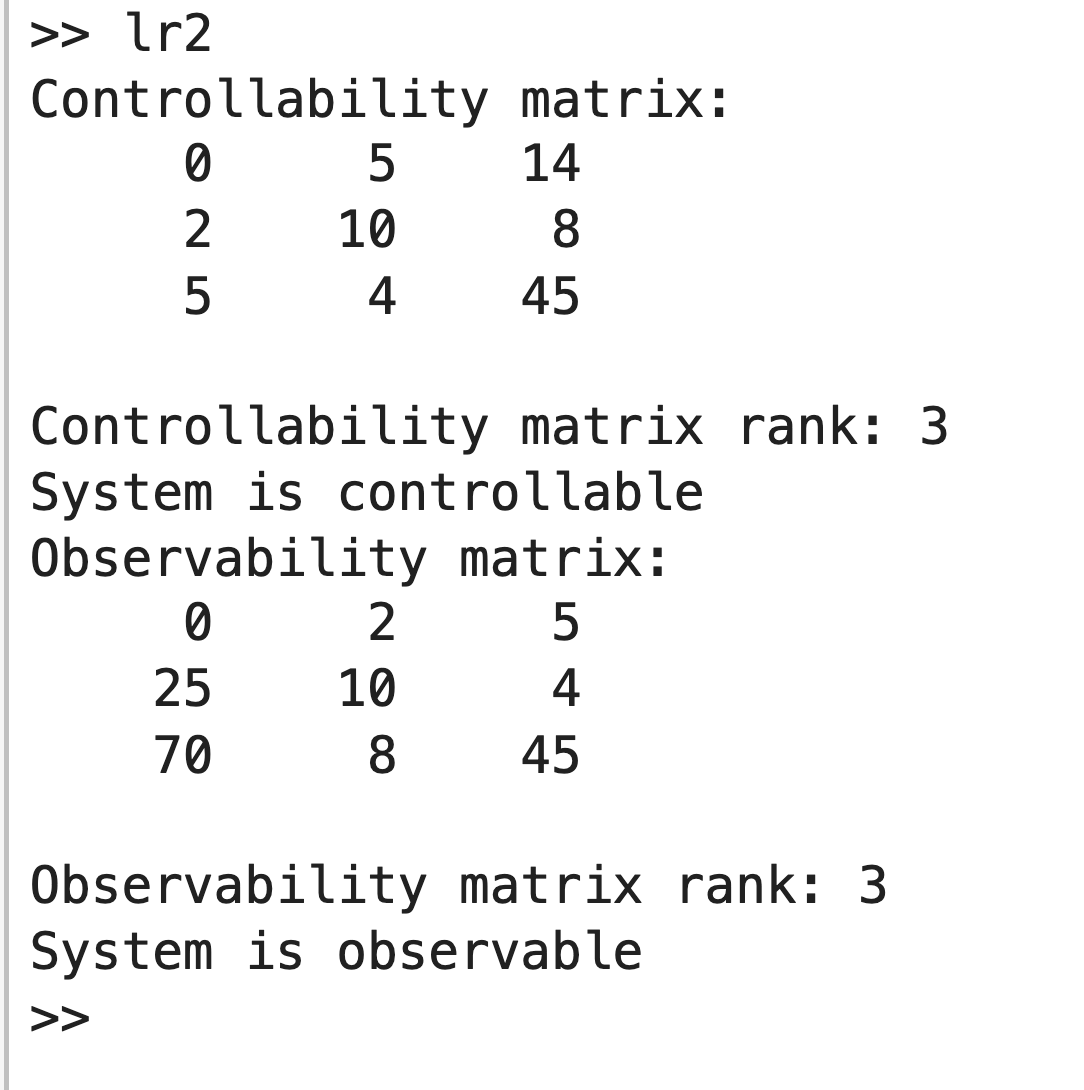
\includegraphics[width=0.5\textwidth]{2.png}
  \caption{The output of controllability and observability.}
\end{figure}

\subsection*{Discussion}
\addcontentsline{toc}{subsection}{Discussion}
This experiment clearly illustrated the use of MATLAB for analyzing the fundamental properties of a dynamic system represented in state-space form. By employing the \texttt{ctrb()} function, we constructed the controllability matrix and verified that the system is fully controllable via its inputs. Similarly, the observability matrix, determined using the \texttt{obsv()} function, was found to have full rank, confirming that the internal states of the system can be inferred from its outputs. These results are crucial for the design of controllers and observers, which are integral to applications such as autonomous robotics and industrial automation.

\subsection*{Conclusion}
\addcontentsline{toc}{subsection}{Conclusion}
The analysis confirmed that the system satisfies the essential criteria for controllability and observability, which are prerequisites for implementing state feedback control. MATLAB’s built-in functions streamlined the verification process, underscoring its effectiveness as a tool for control system analysis and design.


\bibliographystyle{IEEEtran}
\renewcommand{\bibname}{References}
\addcontentsline{toc}{section}{References}
\bibliography{ref}

\end{document}
